\documentclass[10pt]{article}
\usepackage[margin=1in]{geometry}
\usepackage[T1]{fontenc}
\usepackage{lmodern,amsmath,amssymb,booktabs,graphicx,microtype,float}
\usepackage[hidelinks]{hyperref}
\usepackage{natbib}
\setlength{\parskip}{2pt}
\setlength{\emergencystretch}{2em}
\newcommand{\PanelRows}{20,377}
\newcommand{\PanelKeys}{1,214}
\newcommand{\EligibleCases}{22,868}
\newcommand{\ObservedCases}{18,226}
\newcommand{\RepricingRows}{3,665}
\newcommand{\RepricingProviderMonths}{93}
\newcommand{\TimingMatches}{17,065}
\newcommand{\TimingFuturePercent}{98.7}
\newcommand{\DemandOneError}{0.0206}
\newcommand{\DemandOneUSD}{0.054}
\newcommand{\DemandOneSame}{90.7}
\newcommand{\DemandOneRepeat}{22.5}
\newcommand{\DemandThreeError}{0.0618}
\newcommand{\DemandThreeUSD}{0.163}
\newcommand{\DemandThreeSame}{75.9}
\newcommand{\DemandThreeRepeat}{20.0}
\newcommand{\DemandSixError}{0.1342}
\newcommand{\DemandSixUSD}{0.342}
\newcommand{\DemandSixSame}{58.4}
\newcommand{\DemandSixRepeat}{20.4}
\newcommand{\SpotOneError}{0.1429}
\newcommand{\SpotOneUSD}{0.194}
\newcommand{\SpotOneSame}{34.0}
\newcommand{\SpotOneRepeat}{3.2}
\newcommand{\SpotThreeError}{0.2389}
\newcommand{\SpotThreeUSD}{0.290}
\newcommand{\SpotThreeSame}{22.3}
\newcommand{\SpotThreeRepeat}{2.1}
\newcommand{\SpotSixError}{0.2968}
\newcommand{\SpotSixUSD}{0.341}
\newcommand{\SpotSixSame}{14.6}
\newcommand{\SpotSixRepeat}{2.6}

\newcommand{\TimingBlockLower}{23.9}
\newcommand{\TimingBlockUpper}{63.6}
\newcommand{\TimingLooLower}{37.5}
\newcommand{\TimingLooUpper}{44.8}

\hypersetup{pdftitle={Forecasting GPU Rental Prices from Public Catalogs: Why Information Timing and Service Matching Matter}, pdfauthor={H. Esad Kay}, pdfsubject={Research preprint on GPU rental forecast evaluation}}
\title{Forecasting GPU Rental Prices from Public Catalogs:\\Why Information Timing and Service Matching Matter}
\author{H. Esad Kay}
\date{October 29, 2026}
\begin{document}
\maketitle
\begin{abstract}

Public GPU rental catalogs record advertised prices, but their dates do not necessarily show when a forecaster could have used them. This study examines how information timing, service matching, and missing prices affect the evaluation of GPU rental forecasts. It uses 37 public A100, H100, and H200 catalog snapshots from August 2023 to September 2026. A protocol fixed before evaluation compares five methods over one-, three-, and six-month horizons, matching the same observable service over time. Of 22,868 eligible forecasts, 18,226 have an observed target price.

The central result comes from a separate month-start comparison. When later archives are incorrectly treated as available at the start of their nominal month, the one-month on-demand mean absolute log error (MALE) of persistence falls from 0.0353 to 0.0205, an apparent improvement of 42.0\% on the same forecast cases. Persistence simply predicts that the latest available price will remain unchanged. The improvement therefore comes from access to later information, not a better method. An exploratory calendar-block interval for the reduction is 23.9-63.6\%, based on 18 scored forecast origins.

Under the primary availability rules, persistence has the lowest provider-balanced error in all six market-horizon comparisons. However, 90.7\% of its balanced one-month on-demand targets have unchanged prices, and its advantage does not hold uniformly when prices change. A separate post-result change-frequency benchmark does not outperform persistence. Missing targets, stricter service matching, and sparse long-horizon H200 data limit the conclusions. The study extends existing catalog reconstruction into a controlled forecast-evaluation audit. Its findings describe sampled catalog prices, not executable transactions or universal model superiority.

\end{abstract}

\noindent\textbf{Keywords:} GPU rental prices; compute markets; rolling-origin forecasts; catalog data; information timing.\\
\noindent\textbf{Research artifact:} preprint. Empirical data cutoff: September 2026. Sources retrieved: October 28, 2026.\\
\noindent\textbf{Code and results:} \url{https://github.com/esadomer/gpu-rental-backtest-audit}\par
\section{Introduction}

A GPU label alone does not identify a rental service. An A100, for example, may be offered in a single-GPU virtual machine or a multi-GPU server, with different CPU, memory, and interruption conditions. An advertised hourly price therefore applies to a service bundle. If that bundle changes, a difference between two prices may reflect a different product rather than a price change.

This paper asks how accurately an earlier catalog record can predict a future advertised price for the same observable service. The data come from public catalogs that combine offers from several providers. A snapshot is a saved version of such a catalog. The study forecasts the price recorded in a later snapshot; it does not observe a completed rental transaction. Nor does a catalog timestamp establish that the provider refreshed the price, that capacity was immediately available, or that the market first learned the price at that time.

Three terms organize the analysis. The forecast origin is the time at which a prediction is made. The horizon is how many calendar months ahead it looks. The target is the later catalog price against which the prediction is evaluated. An input is admissible only if the archive timestamp used as a proxy for availability is no later than the forecast origin. These definitions make it possible to ask whether a backtest uses information that was actually eligible at the time.

The clearest result holds the forecasting rule and target cases fixed while changing the information allowed at month-start. The rule is persistence: predict the latest admissible price. If archives published later in the month are incorrectly made available on the first day, one-month on-demand mean absolute log error falls by 42.0\%. This error measure compares the logarithms of predicted and observed prices; smaller values are better. The apparent gain measures a distortion in the information set, not an improvement in forecasting skill.

The contribution is an audit of forecast evaluation. It combines rolling forecasts, training outcomes that have become observable before use, comparisons on identical target cases, and explicit records of forecasts that cannot be scored. Earlier work already reconstructs historical GPU prices and identifies timing, identity, and stale-data problems. Here the question is what those records can support when used to evaluate predictions of future prices. The five fixed methods provide reference comparisons; the contribution does not depend on finding a new forecasting algorithm.

Persistence is difficult to beat in this sample, even after repeated provider tables are removed. That result has a limited scope. The history is short, evaluation includes only services with observable targets, catalog entries may be stale, and the model set is deliberately small. Stricter matching of service attributes also removes much of the usable history. These constraints are part of the findings and must be considered alongside forecast accuracy.

\section{Related work and scope}

GPU spot-price forecasting predates the accelerator generations studied here. \citet{khan2022} compare autoregressive, ARIMA, exponential smoothing, and GARCH methods. This paper does not reproduce their experiment, and its five simple specifications do not represent the full range of models in that work. It examines newer public catalogs covering multiple providers, with particular attention to which records may legitimately enter a forecast.

The closest data predecessor is \citet{mittal2026}. Its public repository reconstructs cloud GPU price histories from versioned sources and documents measurement problems. The monthly panel in a pinned revision supplies the archive identifiers used here. This study independently parses forecast prices from the original archives. It does not use the predecessor's cleaned index, retrospective price filters, or backfilled rows as features that would have been available at the forecast date. The two projects serve different research purposes; this distinction is not a claim that the historical dataset is defective.

Mittal's public materials already discuss publication and effective dates, late snapshots, stale provider files, entity matching, matched-item indexes, and survivorship. They also apply publication-date filters when analyzing GPU selection with information available at the time. These ideas are not new claims of this paper. The inspected code and reports did not contain the fixed rolling forecast experiment or the matched-case 42.0\% timing comparison reported here. A renewed audit on October 28, 2026 found that the current public revision matched the pinned release. However, no full manuscript was accessible, so novelty relative to the described paper under review remains uncertain. The project repository records the overlap assessment at the file-path level.

\citet{bandisu2026} study compute asset pricing and the implications of non-storable compute for spot-futures relationships. This catalog study neither estimates their risk premium nor reproduces their synthetic futures. Predictable advertised prices alone do not establish an executable trading strategy. The rolling-origin design and simple benchmarks follow standard forecasting practice \citep{hyndman2021}. Repeated observations across services and the small number of time blocks require caution when drawing statistical conclusions \citep{cameron2015}.

The original project also examined purchase prices for new physical GPUs. The available retail histories did not establish historical product condition and seller continuity for a comparable A100/H100/H200 panel. The present analysis therefore includes neither a physical-price variable nor a synthetic backtest of physical prices. The accompanying research files retain that audit, but it does not establish a purchase-to-rental relationship.

\section{Data and service matching}

\subsection{Archive selection and availability}

The sample contains 37 public gpuhunt ZIP archives \citep{gpuhunt}. They were selected using the monthly snapshot identifiers in the pinned revision of \citet{mittal2026}. The first archive is dated August 28, 2023, September 2023 is absent, and the last archive is dated September 1, 2026. This is a retrospective monthly sample, not a complete list of files that a user could have downloaded at each historical date.

For every archive, the source manifest records its URL, retrieval time, SHA-256 checksum, embedded version, and HTTP S3 Last-Modified timestamp. The analysis uses Last-Modified as a proxy for when that archived object was available. A proxy is an indirect indicator: this timestamp does not prove when public access began, when a provider updated its data, or when market participants could first know a price. All timing conclusions depend on this choice. A sensitivity check adds 24 hours to allow for a small publication delay.

The parser retains the exact accelerator labels A100, H100, and H200 and distinguishes their reported GPU memory. It excludes GH200, H100NVL, and other labels. GCP and RunPod are also excluded because the earlier audit found unresolved historical price-classification or service-tier ambiguities in their common fields. These decisions use metadata evidence, not future forecast performance. The retained economic providers are AWS, Azure, Lambda, DataCrunch/Verda, Nebius, and OCI.

DataCrunch and Verda occur as separate provider files in nine archives from 2026. Their normalized core offer tables are identical in full, and all 810 Verda records for the target GPUs match DataCrunch exactly. Verda's rebranding notice confirms corporate continuity \citep{verda2025}. The model keeps the longer DataCrunch source history and excludes the duplicated Verda records, while the inventory retains both source files. It does not join service histories across the two names.

This provider correction was made after the first model run and is disclosed in a protocol amendment. The original protocol and initial summaries remain available. The predecessor's public data notes also document the relationship between the names.

The cleaning process removes 810 duplicated alias records, 2,847 conflicting records with the same identity in the same snapshot, 28 exact duplicate captures, and 39 target records with invalid numeric values. The resulting panel contains 20,377 service-month records and 1,214 core service identities. Across the panel, 3,665 successive records for the same key show a price change, spread across 93 provider-months. These counts describe records and changes; neither individual rows nor provider-months necessarily represent independent economic events.

\subsection{What the price and service key represent}

The price is the catalog's hourly instance quote in USD divided by the number of GPUs. It includes the host resources supplied with the instance. It is neither the rental price of a bare accelerator nor the resale value of hardware. Provider-specific aggregation also matters. For example, the predecessor documentation describes gpuhunt AWS spot prices as the minimum across availability zones within a region, rather than an executable quote for a particular zone.

A service key is the set of recorded attributes used to match an offer across snapshots. The primary key contains the provider, location, instance name, accelerator name and memory, GPU count, CPU count, host RAM, and spot/on-demand status. Numbers are represented by exact canonical decimal strings. Text identifiers are trimmed, without inferring aliases or ignoring differences in letter case. Records with nonpositive or invalid required numbers are excluded. If one archive lists multiple prices for the same key, those conflicting records are rejected; the parser does not choose the cheapest price.

Disk size and CPU architecture appear inconsistently as the archive schema changes. The primary key therefore uses fields available from the earliest schema. A stricter sensitivity analysis adds disk size and CPU architecture. Missing values remain unknown, and changes in reporting break a service's history under this stricter definition. Even the recorded attributes do not capture every contract term: networking, storage performance, duration, support, taxes, and physical form factors may differ. Matching establishes comparability on observed attributes, not a certified identical service contract.

\subsection{Repeated provider tables and stale data}

Each provider file has two fingerprints. One is a checksum of the raw bytes. The other represents its normalized, sorted core offer table, including prices. The second fingerprint is unchanged by row order, alternative numerical spellings, or added optional fields. It covers all offers in the provider file, not only the target GPUs.

An identical provider table in successive snapshots may reflect unchanged offers, an upstream data feed that has not been refreshed, or both. The archives generally cannot distinguish these explanations. The primary analysis keeps repeated tables because its target is the published aggregate-catalog state. A conservative sensitivity check removes repeated states from both the history and the targets. A changed table still does not prove that every offer was refreshed. Because the check changes both the sample and its history, its error difference cannot be interpreted as the causal effect of stale data.

\section{Forecast evaluation}

The machine-readable protocol was fixed after the source audit and before forecast performance was calculated. It was not publicly preregistered. Two subsequent corrections were documented: the provider-alias correction and a reporting correction that made diagnostic-rate weights consistent with error weights. These were recorded after implementation review. The resulting accuracy ranking was not used to select a model or tune a parameter.

\subsection{When forecasts are made and how targets are selected}

The primary evaluation makes forecasts at 00:00 UTC on the eighth day of each month, beginning in January 2025. An input archive is eligible only if its availability proxy is no later than that forecast origin. Each evaluated service must have 12 earlier observations, and its most recent quote must be no more than 45 days old. Missing months are allowed. Trend calculations use elapsed time, so a gap is not treated as if two observed months were adjacent. A separate sensitivity analysis lowers the history requirement to six observations.

For a horizon $h\in\{1,3,6\}$, the target is the same service key's quote in the selected archive for month $t+h$. That archive must have been available by the eighth day of the target month. This date is the target cutoff. A missing archive, a late archive, or an absent service key leaves the target missing. The evaluation never substitutes the last known price for a missing target.

Forecasts whose target month falls after September 2026 are excluded before evaluation. All other missing outcomes remain in the count of eligible forecasts. Among observed targets, publication occurs approximately 21-27 days after the origin at the one-month horizon, 82-88 days at three months, and 174-177 days at six months. The horizons are therefore calendar-month labels, not exact 30-, 90-, or 180-day realizations. The target is a sampled price at the horizon, not the total cost of renting throughout that period. Two late target archives in 2026 also leave entire origin months unscored in several comparisons.

\subsection{The five forecasting methods}

Let $p_{i,s}$ be the latest admissible price for service i, with log price $\ell_{i,s}=\log p_{i,s}$. Four methods extrapolate only that service's own history:

\begin{itemize}
\setlength{\itemsep}{2pt}
\item Persistence predicts the latest price: $\widehat p_{i,t+h}=p_{i,s}$. It is the no-change benchmark.
\item Drift extends the average log-price change from the first observed price to the last, measured per elapsed month.
\item Local trend fits an ordinary least squares (OLS) slope to log prices over the last 12 observations, using elapsed months. It projects that slope forward from the latest price.
\item Damped trend uses the same local slope but multiplies its projected contribution by 0.5.
\end{itemize}

These are fixed reference specifications, not an exhaustive comparison of classical forecasting methods. The fifth method, pooled ridge, combines training examples across services. It predicts the log return from the latest admissible price to the target directly:

\begin{equation}
 y_{i,t,h}=\log p_{i,t+h}-\log p_{i,s},\qquad
 (\widehat\alpha_h,\widehat\beta_h)=\arg\min_{\alpha,\beta}
 \sum_{j\in\mathcal T_{t,h}} w_j(y_j-\alpha-z_j^\top\beta)^2+0.1\|\beta\|_2^2.
\end{equation}

In equation (1), $z$ contains the seven predictors, $w$ gives the training weights, and $\mathcal T_{t,h}$ is the training set available at origin $t$ for horizon $h$. The predictors are the latest log return per elapsed month, the local log-price slope, the standard deviation of recent log returns per elapsed month, the log of the current price, the log of GPU count, the log of GPU memory, and a spot indicator. Predictors are standardized using weighted training means and variances. The ridge penalty is fixed at 0.1, and the intercept is not penalized.

Training pools accelerator families and the two markets but fits a separate model for each horizon. Each training origin receives equal total weight. Within an origin, providers receive equal weight; within each provider-origin group, examples receive equal weight. Thus a provider with many catalog rows does not dominate training simply because it has more rows.

Training examples may have only four historical observations, whereas the primary evaluation still requires twelve. A training label is the observed outcome for an earlier forecast. It becomes usable only after both the archive's actual publication proxy and the target cutoff have passed, or coincide with the current origin. Training requires at least six such matured training-origin months and 30 examples. If either requirement fails, the model explicitly falls back to persistence. No evaluated primary case needs this fallback.

A provider-holdout sensitivity check removes the evaluated provider's labels from training but retains that provider's observed lagged features as inputs. It tests a conditional form of transfer across providers, not forecasting for a provider with no observed history.

All extrapolated log returns are clipped to $[-\log 10,\log 10]$ relative to the latest price. This predetermined bound prevents extreme numerical extrapolation and is disclosed explicitly; it never activates in the primary evaluation. Empirical price series are never generated synthetically. Synthetic data are used only in software tests.

\subsection{Error measures, missing targets, and uncertainty}

The main measure is mean absolute log error (MALE). For each forecast, it takes the absolute difference between the logarithms of the predicted and observed prices. Within each market and horizon, errors are then averaged in three stages: equally across matched services within each provider-origin group, equally across providers at that origin, and equally across scored origins. For method m and horizon h:

\begin{equation}
 L_{m,h}=\frac{1}{|T|}\sum_{t\in T}\frac{1}{|P_t|}\sum_{a\in P_t}
 \frac{1}{|I_{a,t}|}\sum_{i\in I_{a,t}}
 \left|\log\widehat p^{(m)}_{i,t+h}-\log p_{i,t+h}\right|.
\end{equation}

Here T is the set of scored origin months, $P_t$ is the set of providers represented at origin t, and $I_{a,t}$ contains their matched services for provider a. This provider-balanced calculation prevents a provider with many regional rows from automatically receiving more total weight. The represented providers can change from one origin to the next, so the evaluation is a repeated cross-section of eligible surviving services, not a fixed market portfolio. GPU/VRAM-specific tables use the same weighting.

Mean absolute error (MAE) in dollars per GPU-hour is a secondary measure. MALE is not mean absolute percentage error (MAPE), and its value is not reported as a literal percentage error in price. A percentage reduction in MALE describes improvement in the error measure itself.

Within each specification, all five methods are scored on exactly the same observed targets. The missing-target rate is the raw number of missing targets divided by the number of eligible forecasts. Rates of unchanged prices and repeated provider tables instead use the same nested weights as MALE; raw-row versions are also retained. Accuracy evaluation remains conditional on observing the target. The results do not establish forecast accuracy for services that disappear from the catalog.

For uncertainty checks, each origin supplies a paired error difference: the alternative method's error minus persistence's error. Exploratory 95\% circular moving-block intervals resample the full monthly calendar, including unscored origins, in blocks of length $\max(3,h)$. The calculation uses 2,000 replications and a fixed random seed. Intervals are not reported if the number of observed origins is less than four times the block length. In particular, the headline six-month comparisons have too few time blocks. These intervals and the leave-one-provider-out summaries describe stability within the data; they do not establish strong population inference or significance based on independent trades.

\section{Main results}

\subsection{Coverage and the no-change benchmark}

Across the three horizons, 22,868 service-origin-horizon forecasts meet the eligibility rules and 18,226 have observed targets (Table 1). The same service can contribute several overlapping forecasts. Missing-target rates range from 14.5\% to 19.8\% for on-demand and from 31.5\% to 39.0\% for spot. H200 has particularly little long-horizon history: only four on-demand six-month cases and no spot six-month cases meet the primary matching rules. The four observed cases are not four independent economic events.

\begin{table}[H]
\centering\small
\begin{tabular}{lrrrrrrr}
\toprule
Market & $h$ & Eligible & Observed & Months & Prov. & Missing & Same \\
\midrule
On Demand & 1 & 7,031 & 6,015 & 18 & 6 & 14.5\% & 90.7\% \\
On Demand & 3 & 6,094 & 5,103 & 16 & 6 & 16.3\% & 75.9\% \\
On Demand & 6 & 4,800 & 3,848 & 13 & 6 & 19.8\% & 58.4\% \\
Spot & 1 & 2,046 & 1,402 & 18 & 4 & 31.5\% & 34.0\% \\
Spot & 3 & 1,674 & 1,112 & 16 & 3 & 33.6\% & 22.3\% \\
Spot & 6 & 1,223 & 746 & 13 & 3 & 39.0\% & 14.6\% \\
\bottomrule
\end{tabular}

\caption{Primary coverage. Months counts origins with scored forecasts; Prov. counts distinct economic providers represented in the comparison. Missing is the raw missing-target rate among eligible cases. Same is the provider-balanced share of observed targets whose prices do not change. Counts are not independent sample sizes.}
\label{tab:table1}
\end{table}

Persistence has the lowest aggregate MALE in all six market-horizon comparisons (Table 2). At one month, its dollar MAE is \$0.054 per GPU-hour for on-demand and \$0.194 for spot. These results apply to the selected services whose target prices remain observable; they are not a guarantee for a current quote or workload.

\begin{table}[H]
\centering\small
\begin{tabular}{lrrrrrr}
\toprule
Market & $h$ & Persist. & Drift & Trend & Damped & Ridge \\
\midrule
On Demand & 1 & 0.0206 & 0.0337 & 0.0362 & 0.0284 & 0.0318 \\
On Demand & 3 & 0.0618 & 0.0882 & 0.0944 & 0.0778 & 0.0913 \\
On Demand & 6 & 0.1342 & 0.1739 & 0.1810 & 0.1552 & 0.1708 \\
Spot & 1 & 0.1429 & 0.1680 & 0.1753 & 0.1570 & 0.1520 \\
Spot & 3 & 0.2389 & 0.3013 & 0.3314 & 0.2767 & 0.2623 \\
Spot & 6 & 0.2968 & 0.4550 & 0.5178 & 0.3907 & 0.3282 \\
\bottomrule
\end{tabular}

\caption{Mean absolute log error, with origins and providers equally weighted at their respective levels. Lower values indicate smaller errors. Damped trend uses a fixed 0.5 slope contribution; ridge uses a fixed penalty. The results were not used to select a model.}
\label{tab:table2}
\end{table}

\begin{figure}[H]
\centering
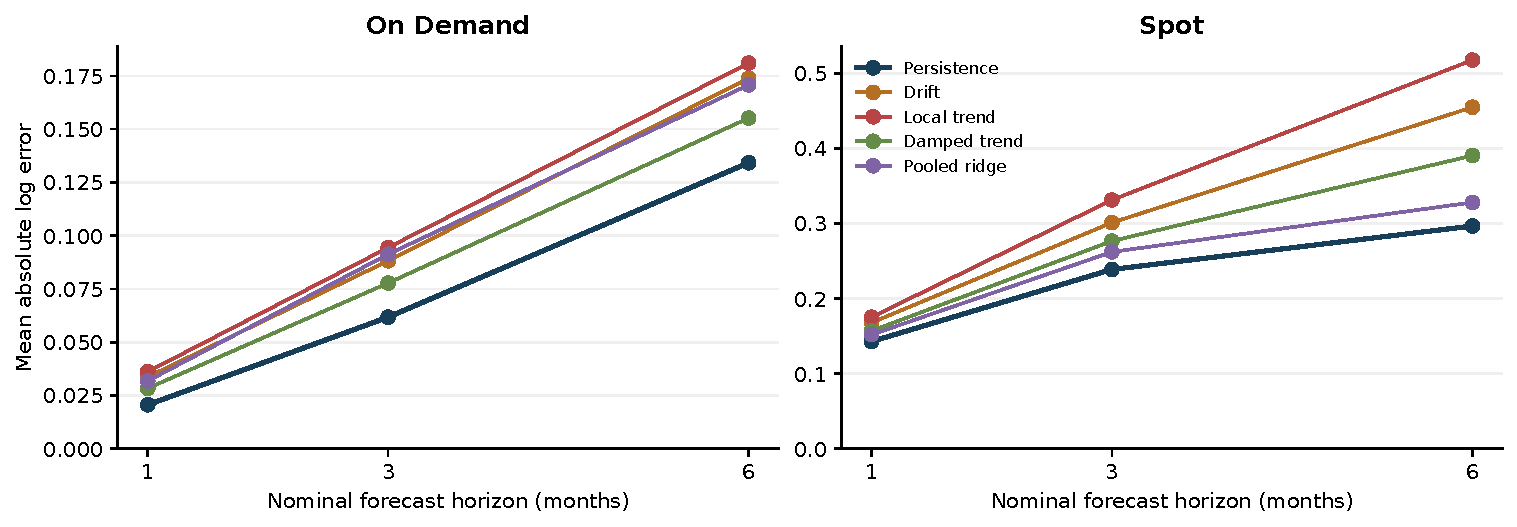
\includegraphics[width=\linewidth]{figures/forecast_errors.pdf}
\caption{Errors for the five fixed methods. Within each market and horizon, every method uses the same observed targets. Six-month comparisons contain only 13 scored origins, and their forecast periods overlap.}
\label{fig:figure1}
\end{figure}

Much of the one-month on-demand sample does not change price. Unchanged targets account for 90.7\% of its balanced target weight, compared with 34.0\% for spot. Entire provider tables repeat for 22.5\% and 3.2\% of those respective balanced target populations. Figure 2 distinguishes three phenomena: a particular price can remain unchanged, a whole provider table can repeat, or a target can be missing. None is interchangeable with the others.

\begin{figure}[H]
\centering
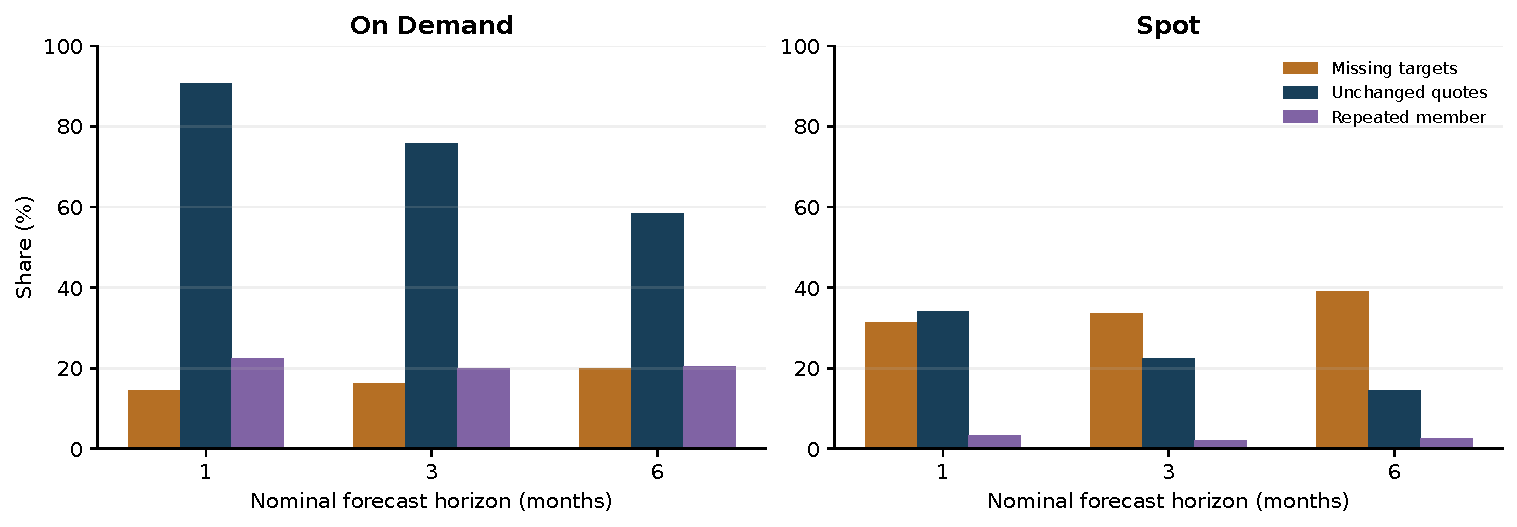
\includegraphics[width=\linewidth]{figures/coverage_limits.pdf}
\caption{Coverage and price repetition. Missing targets are raw fractions of eligible cases. Unchanged prices and repeated provider tables are provider-balanced fractions of observed targets. A repeated table does not prove that prices are stale; a changed table does not prove that each unchanged price was refreshed.}
\label{fig:figure2}
\end{figure}

\subsection{What the sensitivity checks establish}

Removing repeated provider tables leaves persistence first in the aggregate ranking. It also reduces one-month on-demand observed cases from 6,015 to 2,965. Because this changes provider composition and usable history, the error comparison cannot isolate the effect of stale data. Stricter matching on optional service attributes leaves only six scored one-month origins and three scored three-month origins, with no six-month targets. Claims about services held fixed on all these attributes thus have much less data behind them than the primary panel suggests.

\begin{table}[H]
\centering\small
\begin{tabular}{llrrrr}
\toprule
Specification & Market & Cases & Months & Persist. & Ridge \\
\midrule
Primary & On Demand & 6015 & 18 & 0.0206 & 0.0318 \\
Primary & Spot & 1402 & 18 & 0.1429 & 0.1520 \\
Repeated members removed & On Demand & 2965 & 18 & 0.0269 & 0.0396 \\
Repeated members removed & Spot & 1349 & 18 & 0.1508 & 0.1585 \\
Six observations & On Demand & 7689 & 18 & 0.0208 & 0.0320 \\
Six observations & Spot & 2138 & 18 & 0.1566 & 0.1696 \\
Strict identity & On Demand & 1873 & 6 & 0.0229 & 0.0359 \\
Strict identity & Spot & 389 & 6 & 0.1680 & 0.1745 \\
Provider holdout & On Demand & 6015 & 18 & 0.0206 & 0.0376 \\
Provider holdout & Spot & 1402 & 18 & 0.1429 & 0.1517 \\
\bottomrule
\end{tabular}

\caption{Selected one-month sensitivity results. These checks use different samples, except provider holdout, which changes only ridge training. Results for all horizons and methods accompany the study.}
\label{tab:table3}
\end{table}

Adding a 24-hour publication lag changes neither primary cases nor scores under the eighth-day schedule. This tests a small timing delay, not the validity of Last-Modified as an availability proxy. Neither the six-observation sample nor conditional provider holdout reverses persistence's aggregate ranking. The ridge specification therefore provides no established transferable improvement from learning across providers. Leave-one-provider-out and GPU-specific tables are supplied to show how composition varies beneath the aggregate results.

\subsection{How later information makes a forecast look better}

The primary eighth-day schedule allows archives published during the first week to enter the information set. A separate diagnostic moves the forecast origin to the first day of each month. It compares two timing rules on 17,065 identical combinations of service key, origin, horizon, and target. The comparison holds the forecast cases fixed, so changes in error cannot be attributed to a different set of target cases.

The admissible rule uses archived publication times. The deliberately inadmissible rule treats each month's archive as available at the start of its nominal month, even if the archive was published later. For example, an archive published after month-start can then supply an input to a forecast dated at month-start. Both rules still use actual archive dates to calculate elapsed time and the eighth-day cutoff to decide whether a target is observed.

The nominal-label rule uses an input published after the origin in 98.7\% of matched cases. For one-month on-demand forecasts, persistence MALE falls from about 0.0353 to 0.0205, a 42.0\% apparent reduction. The corresponding spot reduction is 33.9\% (Table 4). These percentages describe reductions in forecast error, not changes in rental prices or trading returns. The rule intentionally gives a forecast later information, making it a diagnostic of evaluation bias rather than a valid strategy. The result does not imply that every historical dataset with nominal dates is unusable.

\begin{table}[H]
\centering\small
\begin{tabular}{lrrrr}
\toprule
Market & $h$ & Actual timing & Nominal label & Apparent reduction \\
\midrule
On Demand & 1 & 0.0353 & 0.0205 & 42.0\% \\
On Demand & 3 & 0.0834 & 0.0602 & 27.8\% \\
On Demand & 6 & 0.1474 & 0.1352 & 8.3\% \\
Spot & 1 & 0.2077 & 0.1373 & 33.9\% \\
Spot & 3 & 0.2731 & 0.2425 & 11.2\% \\
Spot & 6 & 0.3051 & 0.2918 & 4.3\% \\
\bottomrule
\end{tabular}

\caption{Persistence under two timing rules on identical matched first-day cases. Actual timing uses the availability proxy. Nominal label permits information published later. Coverage outside the matched intersection is reported separately in the run manifest.}
\label{tab:table4}
\end{table}

\begin{figure}[H]
\centering
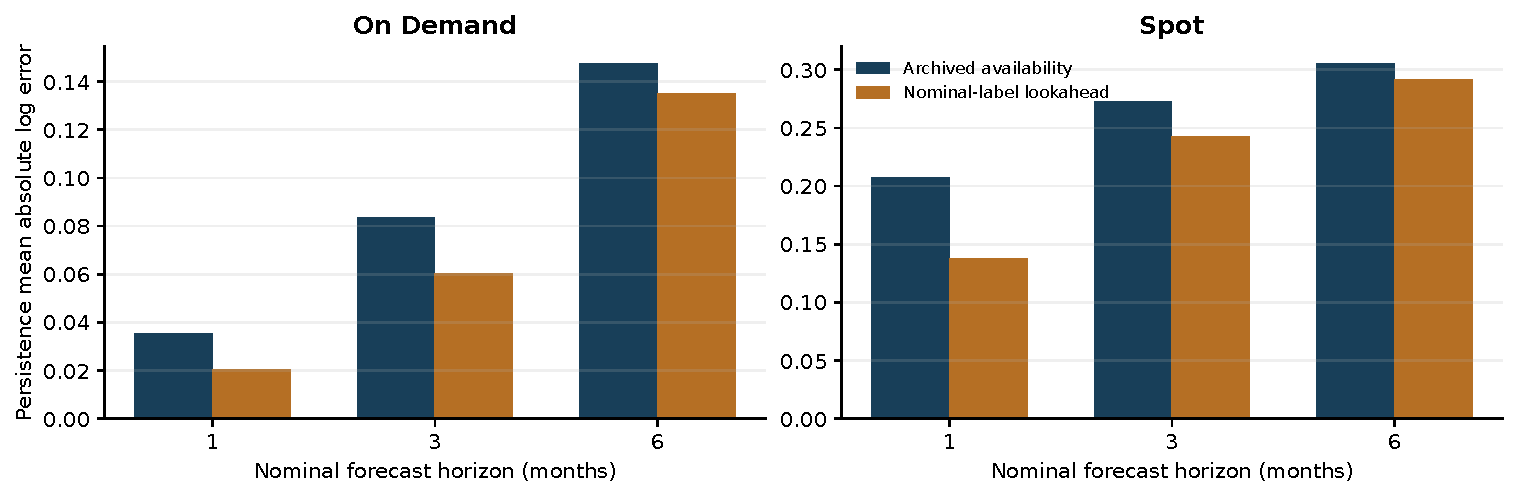
\includegraphics[width=\linewidth]{figures/timing_diagnostic.pdf}
\caption{Sensitivity of the month-start comparison to the permitted information set. These bars do not estimate the accuracy of trades executable on the first day of each month.}
\label{fig:figure3}
\end{figure}

\section{Exploratory checks: timing, price changes, and missing targets}

The analyses in this section were designed after the original results were known. Their separate machine-readable plan was fixed before the additional calculations, but they use the same data and remain exploratory. They are neither preregistered tests nor independent confirmation. The original protocol, five-model results, and analysis audit trail remain available. No new empirical observations or imputed prices enter these analyses.

\subsection{How stable is the 42\% timing result?}

The one-month on-demand comparison contains 5,753 paired cases at 18 scored origins within a 20-month calendar. With three-month blocks and 2,000 paired draws, the exploratory 95\% interval for the relative MALE reduction is [23.9\%, 63.6\%]. The absolute reduction is 0.01485, with interval [0.00425, 0.03091]. Each draw resamples the actual-timing and nominal-label origin losses together, then recalculates the ratio of their mean losses. It does not average origin-specific percentage reductions. The calendar retains the unscored April and June 2026 origins.

Using two- and four-month blocks gives relative intervals of [23.1\%, 67.3\%] and [25.8\%, 61.1\%]. A six-month-block interval is not reported: 18 observed origins fall below the required 24. For other horizons the primary block length remains $\max(3,h)$, and no primary six-month interval is reported. The small number of months, shared shocks, and possible regime changes limit the interpretation of these intervals as confidence intervals with reliable coverage. They describe stability under the chosen resampling scheme, not population significance. No usable draw in a reported interval has a zero baseline loss; the implementation would suppress the relative interval if that occurred.

\begin{table}[H]
\centering\small
\begin{tabular}{lrrrrr}
\toprule
Population & Cases & Months & Actual & Nominal & Reduction \\
\midrule
Full sample & 5,753 & 18 & 0.0353 & 0.0205 & 42.0\% \\
Omit AWS & 5,328 & 18 & 0.0320 & 0.0188 & 41.1\% \\
Omit Azure & 3,942 & 18 & 0.0445 & 0.0260 & 41.6\% \\
Omit DataCrunch & 5,302 & 18 & 0.0223 & 0.0124 & 44.4\% \\
Omit Lambda & 3,647 & 18 & 0.0389 & 0.0243 & 37.5\% \\
Omit Nebius & 5,731 & 18 & 0.0339 & 0.0187 & 44.8\% \\
Omit OCI & 4,815 & 18 & 0.0403 & 0.0226 & 44.0\% \\
2025 origins & 3,312 & 12 & 0.0357 & 0.0202 & 43.5\% \\
2026 origins & 2,441 & 6 & 0.0347 & 0.0211 & 39.1\% \\
\bottomrule
\end{tabular}

\caption{One-month on-demand timing comparison for persistence. Forecasts remain paired within each row's sample. Provider omissions are reweighted; year groups use the forecast-origin year. Every provider-omission row retains 18 origins. Only six scored origins fall in 2026.}
\label{tab:table5}
\end{table}

The apparent reduction remains positive after each provider is omitted, ranging from 37.5\% to 44.8\% (Table 5). This does not mean that every provider individually shows a reduction. Nebius has equal losses under the two timing rules across its three represented origins. OCI has zero loss under both rules, so its relative reduction is undefined. The other providers' reductions range from 37.7\% to 70.9\% over their own observed origins. The reductions for 2025 and 2026 are 43.5\% and 39.1\%. These comparisons change both composition and time coverage, so they do not isolate provider effects or establish a stable economic regime.

\begin{figure}[H]
\centering
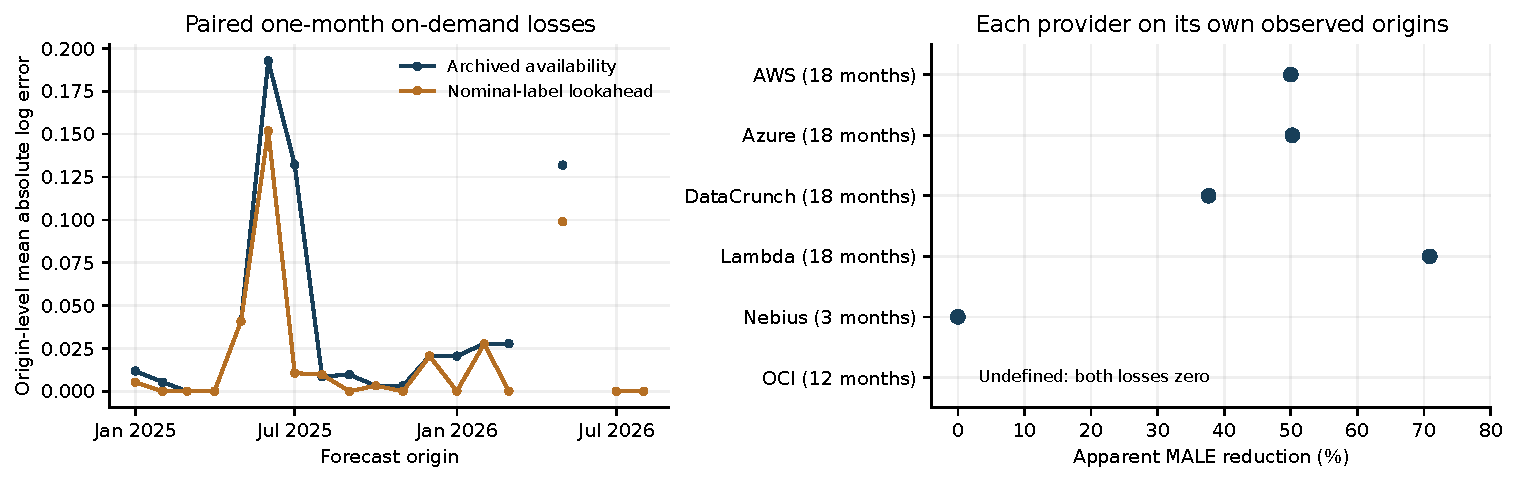
\includegraphics[width=\linewidth]{figures/v3_timing_stability.pdf}
\caption{Detail of the exploratory timing comparison. Left panel: paired origin losses, with unscored months left as gaps. Right panel: each provider evaluated on its own observed origins. Provider percentages are not additive contributions to the full-sample reduction. No percentage is assigned to OCI because both losses are zero.}
\label{fig:figure4}
\end{figure}

Removing each observed origin month in turn leaves 17 origins and gives one-month on-demand reductions from 28.9\% to 51.1\%. Omitting July 2025 produces the minimum; omitting June 2025 produces the maximum. Each result is a recalculated ratio of paired mean losses, not an average of monthly percentages. No model is refitted.

The direction therefore survives every single-origin deletion, but the size depends materially on particular months. July 2025 alone accounts for 45.5\% of the full sample's signed actual-minus-nominal MALE difference. Deleting one origin at a time cannot rule out joint concentration across several months or establish an effect that holds across regimes.

\begin{table}[H]
\centering\small
\begin{tabular}{lrrrlrl}
\toprule
Market & $h$ & Runs & Minimum & Omitted & Maximum & Omitted \\
\midrule
On Demand & 1 & 18 & 28.9\% & 2025-07 & 51.1\% & 2025-06 \\
On Demand & 3 & 16 & 21.2\% & 2025-07 & 32.9\% & 2025-05 \\
On Demand & 6 & 13 & 3.7\% & 2025-07 & 9.7\% & 2025-01 \\
Spot & 1 & 18 & 31.1\% & 2025-01 & 36.2\% & 2026-08 \\
Spot & 3 & 16 & 9.1\% & 2026-06 & 12.7\% & 2026-05 \\
Spot & 6 & 13 & 1.8\% & 2025-06 & 6.7\% & 2025-01 \\
\bottomrule
\end{tabular}

\caption{Timing sensitivity when one observed origin is omitted. Each run removes that origin's complete paired comparison and averages the remaining origin losses equally. The minimum and maximum are relative error reductions, not confidence bounds. Unscored calendar months are not deletion runs. All 94 defined results remain positive, but the runs are dependent diagnostics. Individual runs and retained-case counts are available in the repository.}
\label{tab:table6}
\end{table}

\subsection{Does persistence still perform best when prices change?}

Persistence predicts an unchanged price exactly. Separating changed and unchanged outcomes shows how much its overall performance depends on this property. At one month, the changed on-demand subset contains 423 rows, nine origins, and 12 provider-origin groups. It accounts for 9.3\% of the original balanced target weight but 7.0\% of raw rows. The changed spot subset contains 695 rows and 66.0\% of the balanced target weight. These groups are defined by what happens after the forecast; a forecaster cannot use them to select cases in advance.

The calculation keeps each case's original weight $w_i$ from the full observed market-horizon group. For subgroup C, let $s_C=\sum_{i\in C}w_i$ be its total weight and $L_C=(\sum_{i\in C}w_i e_i)/s_C$ its conditional loss. The overall loss then satisfies $L=s_{\mathrm{changed}}L_{\mathrm{changed}}+s_{\mathrm{same}}L_{\mathrm{same}}$. Thus each subgroup's loss contributes in proportion to its original weight. Rebalancing the subgroups separately would answer a different question and break this decomposition.

\begin{table}[H]
\centering\small
\begin{tabular}{lrrrr}
\toprule
Model & OD changed & OD same & Spot changed & Spot same \\
\midrule
Persistence & 0.2227 & 0.0000 & 0.2166 & 0.0000 \\
Drift & 0.2242 & 0.0143 & 0.2349 & 0.0383 \\
Local trend & 0.2280 & 0.0166 & 0.2465 & 0.0374 \\
Damped trend & 0.2253 & 0.0083 & 0.2284 & 0.0187 \\
Pooled ridge & 0.2209 & 0.0125 & 0.2171 & 0.0260 \\
Frequency-shrunk trend & 0.2234 & 0.0016 & 0.2278 & 0.0078 \\
\bottomrule
\end{tabular}

\caption{One-month conditional MALE using the original observed-group weights. OD means on-demand. Frequency-shrunk trend is the separate exploratory benchmark defined in Section 6.4. Each conditional loss is divided by its subgroup's total weight; the two groups are not treated as equally large. Same denotes unchanged prices.}
\label{tab:table7}
\end{table}

For changed on-demand prices, pooled ridge has a slightly smaller MALE than persistence: 0.2209 versus 0.2227. On unchanged prices, however, ridge has an error of 0.0125 while persistence has zero error. Because unchanged targets carry 90.7\% of the balanced weight, this explains ridge's worse overall score. The small subset, defined after observing outcomes, does not establish changed-case superiority or statistical significance. For changed one-month spot prices, persistence remains best among the original five methods. Its aggregate advantage therefore reflects both the frequency of unchanged prices and model performance when repricing occurs, with different patterns across the two markets.

\subsection{Why are some target prices missing?}

A late archive and an absent service key cause different forms of missingness. Of the 1,016 missing one-month on-demand targets, 901 belong to two late target-month archives, May and July 2026. The other 115 have no matching service key in an otherwise timely archive. Spot missingness is more evenly split: 319 late-archive cases and 325 absent-key cases. The rule checks archive lateness first. A late-archive classification therefore does not establish whether the key was present, and neither classification proves permanent delisting.

\begin{table}[H]
\centering\small
\begin{tabular}{lrrrrr}
\toprule
Market & $h$ & Eligible & Late archive & Absent key & Absent / on-time \\
\midrule
On Demand & 1 & 7,031 & 901 & 115 & 1.9\% \\
On Demand & 3 & 6,094 & 844 & 147 & 2.8\% \\
On Demand & 6 & 4,800 & 817 & 135 & 3.4\% \\
Spot & 1 & 2,046 & 319 & 325 & 18.8\% \\
Spot & 3 & 1,674 & 237 & 325 & 22.6\% \\
Spot & 6 & 1,223 & 173 & 304 & 29.0\% \\
\bottomrule
\end{tabular}

\caption{Sources of missing targets among eligible cases, counted as raw rows. The last column divides absent-key cases by eligible cases after excluding late archives. It measures absence conditional on an on-time archive and does not correct selection bias. Shared archive delays and overlapping forecast horizons mean that rows are not independent failures.}
\label{tab:table8}
\end{table}

Among eligible one-month cases with on-time target archives, absent keys account for 1.9\% of on-demand and 18.8\% of spot cases. Of the 325 absent spot keys, 267 are Azure cases and 58 are DataCrunch cases. At the forecast origin, these absent-key spot cases have a raw mean quote age of 17.7 days and 15.9 historical observations. Observed spot targets have corresponding means of 13.7 days and 18.4 observations. Absent-key on-demand cases have a higher raw mean past repricing frequency than observed cases, 15.5\% versus 4.4\%. These features were known at the origin, but their differences also reflect provider and time composition.

The supplement reports status counts by provider, GPU/VRAM, origin year, and provider/GPU, along with raw feature means and shares under the original eligible-case weights. For example, total one-month on-demand missingness is 14.5\% by raw case counts and 12.0\% under nested eligible-case weights. These denominators differ from the observed-case weights used to score forecast accuracy.

The comparisons show that target observability varies with observed characteristics. They do not reveal the missing prices, prove that missingness is conditionally independent, or establish the direction of any bias in reported forecast error. The study applies neither inverse-probability correction nor a backtest based on invented missing targets.

\subsection{A benchmark that adjusts for past price-change frequency}

The final exploratory benchmark reduces the size of the trend adjustment when a service has rarely changed price. Let $f_{i,t}$ be the fraction of adjacent nominal-month pairs with a price change among the last 12 admissible observations. Pairs separated by missing months are excluded, and all underlying records must have been published by the origin. Define $q_{i,t,h}=1-(1-f_{i,t})^h$. The forecast is then:

\begin{equation}
\log\widehat p^{\mathrm{freq}}_{i,t+h}
=\log p_{i,s}+q_{i,t,h}\bigl(\log\widehat p^{\mathrm{damped}}_{i,t+h}-\log p_{i,s}\bigr).
\end{equation}

Equation (3) moves the original bounded damped-trend forecast toward persistence, with the amount of movement determined by past repricing frequency. The factor q is a shrinkage factor for the nominal horizon, not a calibrated probability that the price will change. The distinction matters because the damped trend uses elapsed time from the latest publication to the target cutoff, whereas h runs from the forecast origin. If a history contains no adjacent pair, the method explicitly falls back to persistence. No evaluated case requires that fallback. The window and formula were fixed before evaluating this supplement, without tuning or searching over alternative formulas.

\begin{table}[H]
\centering\small
\begin{tabular}{lrrrrr}
\toprule
Market & $h$ & Persistence & Damped & Freq.-shrunk & Excess error \\
\midrule
On Demand & 1 & 0.0206 & 0.0284 & 0.0222 & 7.4\% \\
On Demand & 3 & 0.0618 & 0.0778 & 0.0687 & 11.2\% \\
On Demand & 6 & 0.1342 & 0.1552 & 0.1451 & 8.1\% \\
Spot & 1 & 0.1429 & 0.1570 & 0.1529 & 7.0\% \\
Spot & 3 & 0.2389 & 0.2767 & 0.2720 & 13.9\% \\
Spot & 6 & 0.2968 & 0.3907 & 0.3860 & 30.1\% \\
\bottomrule
\end{tabular}

\caption{Exploratory frequency-shrunk benchmark on the original primary observed cases. Excess error is the relative MALE increase over persistence. It is calculated from unrounded scores, before formatting the displayed values. The original five-method experiment is unchanged.}
\label{tab:table9}
\end{table}

The adjustment reduces damped-trend error in all six comparisons, but remains 7.0-30.1\% worse than persistence. This result concerns this particular fixed adjustment; it does not rule out every conditional or event-based model. The full supplement includes paired comparisons under the original horizon-dependent uncertainty rules. Six-month intervals remain unreported.

\section{Interpretation and limitations}

For a compute-pricing desk, a forecast should be accompanied by enough information to interpret it: the service key, source timestamp, age of the latest input, whether the provider table repeats, and the history of missing targets. Persistence provides a useful benchmark in this sample. A more elaborate method should demonstrate improvement under the same information and matching rules. Otherwise, an apparent gain may reflect later data, a different service, or a different set of services with observable targets.

The data impose several limits. All observations come through one public aggregation pipeline; multiple providers do not represent independent collection systems. Archive timestamps are imperfect proxies for availability. Advertised prices do not establish transactions, available capacity, counterparties, execution terms, or interruption costs. Monthly sampling misses price movements within the month, especially in spot markets. Excluding providers with unresolved metadata ambiguity improves interpretability but reduces market coverage.

Service matching is also incomplete. The primary key omits some contract attributes, while the stricter key cannot support a six-month backtest. Long-horizon H200 evidence is sparse. Regional rows may share provider decisions and common time shocks, and overlapping forecast periods reduce the effective information further. Large row counts should not obscure these dependencies.

The model comparison covers four simple time-series methods and one fixed pooled regression. The supplement adds one explicitly disclosed heuristic designed after the original results. This limited set cannot rule out gains from relevant event information, a better specified dynamic model, a longer history, or refreshed provider-native data. Changed-price and missingness checks help explain the sample, but do not repair selection into observable targets.

The error ranking provides no conclusion about causal supply or demand effects, futures risk premia, hardware depreciation, realizable arbitrage, or market efficiency. Public access to sources also does not imply blanket redistribution rights. The reproducibility package therefore separates retrieval instructions from raw third-party archives.

\section{Conclusion}

The main finding is that an evaluation can make an unchanged forecasting rule look substantially better by allowing it later information. In the paired month-start comparison, this alone reduces one-month on-demand persistence error by 42.0\% on the same forecast cases. Exploratory block, provider-omission, origin-year, and single-origin-deletion checks retain the direction of that result. However, the deletion analysis shows substantial concentration in particular months, and the checks cannot exclude joint dependence on several repricing events.

Under the admissible primary schedule, persistence outperforms the fixed alternatives in aggregate. Its advantage is not uniform within changed-price subsets, and the additional frequency-based heuristic does not reverse the aggregate ranking. Missing targets arise both from shared archive delays and absent service keys; forecast errors for those missing outcomes remain unknown.

Forecast accuracy in these catalogs must therefore be read together with information timing, observable service identity, unchanged prices, repeated provider tables, and missing outcomes. The study extends earlier historical reconstruction into a controlled forecast audit. It neither claims first discovery of the underlying data problems nor establishes that compute prices are universally unforecastable. Sparse long-horizon H200 coverage remains a firm limit on the evidence.

\appendix
\section{Reproduction and audit trail}

The public project is available at \url{https://github.com/esadomer/gpu-rental-backtest-audit}. It contains the original locked protocol, the provider-alias amendment made after the first run, source manifests, extraction and evaluation scripts, behavioral tests, supplementary analyses, aggregate results, and manuscript source. Downloadable source and reproducibility packages accompany the compiled preprint.

The supplied commands retrieve the registered public inputs and regenerate every eligible forecast case, including cases with missing targets. They then reproduce the timing, conditional-loss, attrition, frequency-benchmark, and origin-deletion diagnostics. Neither raw third-party archives nor row-level outputs are bundled in the repository or reproducibility package. The protocol SHA-256 is:

\begin{center}\scriptsize\texttt{6d3f44cede6f791542aeed2425f5325b85c01f0a2c3bf119e045f77b4a6574e5}\end{center}

Run manifests fingerprint the amended method, archived inputs, and research code. The supplementary analyses have their own post-result plans, freeze records, and run manifests. A preserved base-run reference authenticates the original scientific fields while allowing fresh reproduction timestamps, runtime metadata, and additional script entries. Original code and empirical input hashes remain pinned. Raw downloads are retained locally and are excluded from the manuscript-source archive.

The README specifies the environment and commands for archive retrieval, rolling evaluation, independent result verification, and figure generation. The empirical inputs required no paid feed, private account, or vendor request. Synthetic test fixtures check future-data exclusion, missing targets, decimal-based identity, duplicated provider files, training-label maturity, provider holdout, nested weights, and uncertainty on sparse calendars. They never enter empirical output files.

\clearpage
\begin{thebibliography}{9}
\bibitem[Bandi and Su(2026)]{bandisu2026}
F. M. Bandi and Y. Su. (Early) AI Compute Asset Pricing. \emph{arXiv:2607.12156v4}, 2026. \url{https://arxiv.org/abs/2607.12156v4}.
\bibitem[Cameron and Miller(2015)]{cameron2015}
A. C. Cameron and D. L. Miller. A practitioner's guide to cluster-robust inference. \emph{Journal of Human Resources}, 50(2):317--372, 2015. \url{https://doi.org/10.3368/jhr.50.2.317}.
\bibitem[dstack(gpuhunt)]{gpuhunt}
dstack. \emph{gpuhunt: GPU prices aggregator for cloud providers}. Public software and versioned catalog infrastructure. \url{https://github.com/dstackai/gpuhunt}. Archives accessed October 28, 2026; exact object URLs and checksums are listed in the source manifest.
\bibitem[Hyndman and Athanasopoulos(2021)]{hyndman2021}
R. J. Hyndman and G. Athanasopoulos. \emph{Forecasting: Principles and Practice}, third edition. OTexts, 2021. Chapter 5. \url{https://otexts.com/fpp3/toolbox.html}.
\bibitem[Khan et al.(2022)]{khan2022}
M. Khan, A. I. Jehangiri, Z. Ahmad, M. A. Ala'anzy, and A. Umer. An exploration to graphics processing unit spot price prediction. \emph{Cluster Computing}, 25:3499--3515, 2022. \url{https://doi.org/10.1007/s10586-022-03581-8}.
\bibitem[Mittal(2026)]{mittal2026}
R. Mittal. \emph{gpu-price-history}. Public reconstruction repository and accompanying manuscript description, 2026. Pinned revision \texttt{ee8820dd90d7715d8bb57cee03fb0882706d76c5}. \url{https://github.com/rahilmittal1/gpu-price-history}. Repository-generated data are attributed under CC BY 4.0; original third-party archives retain their own terms.
\bibitem[Verda(2025)]{verda2025}
Verda. DataCrunch is changing its name to Verda. November 5, 2025. \url{https://verda.com/blog/datacrunch-is-changing-its-name-to-verda}.
\end{thebibliography}
\end{document}
